\section{PS0: Hello SFML}\label{sec:ps0}

\subsection{Discussion}\label{sec:ps0:disc}

This project was intended to introduce SFML, emphasizing the setup of Visual Studio Code as the development environment. We started with a provided codebase showcasing a green circle and were challenged to enhance the experience by introducing a sprite texture. The objective is to gain practical experience with SFML's features and attributes while customizing the code in a familiar IDE.


\begin{figure}[tbh]
	\centering
	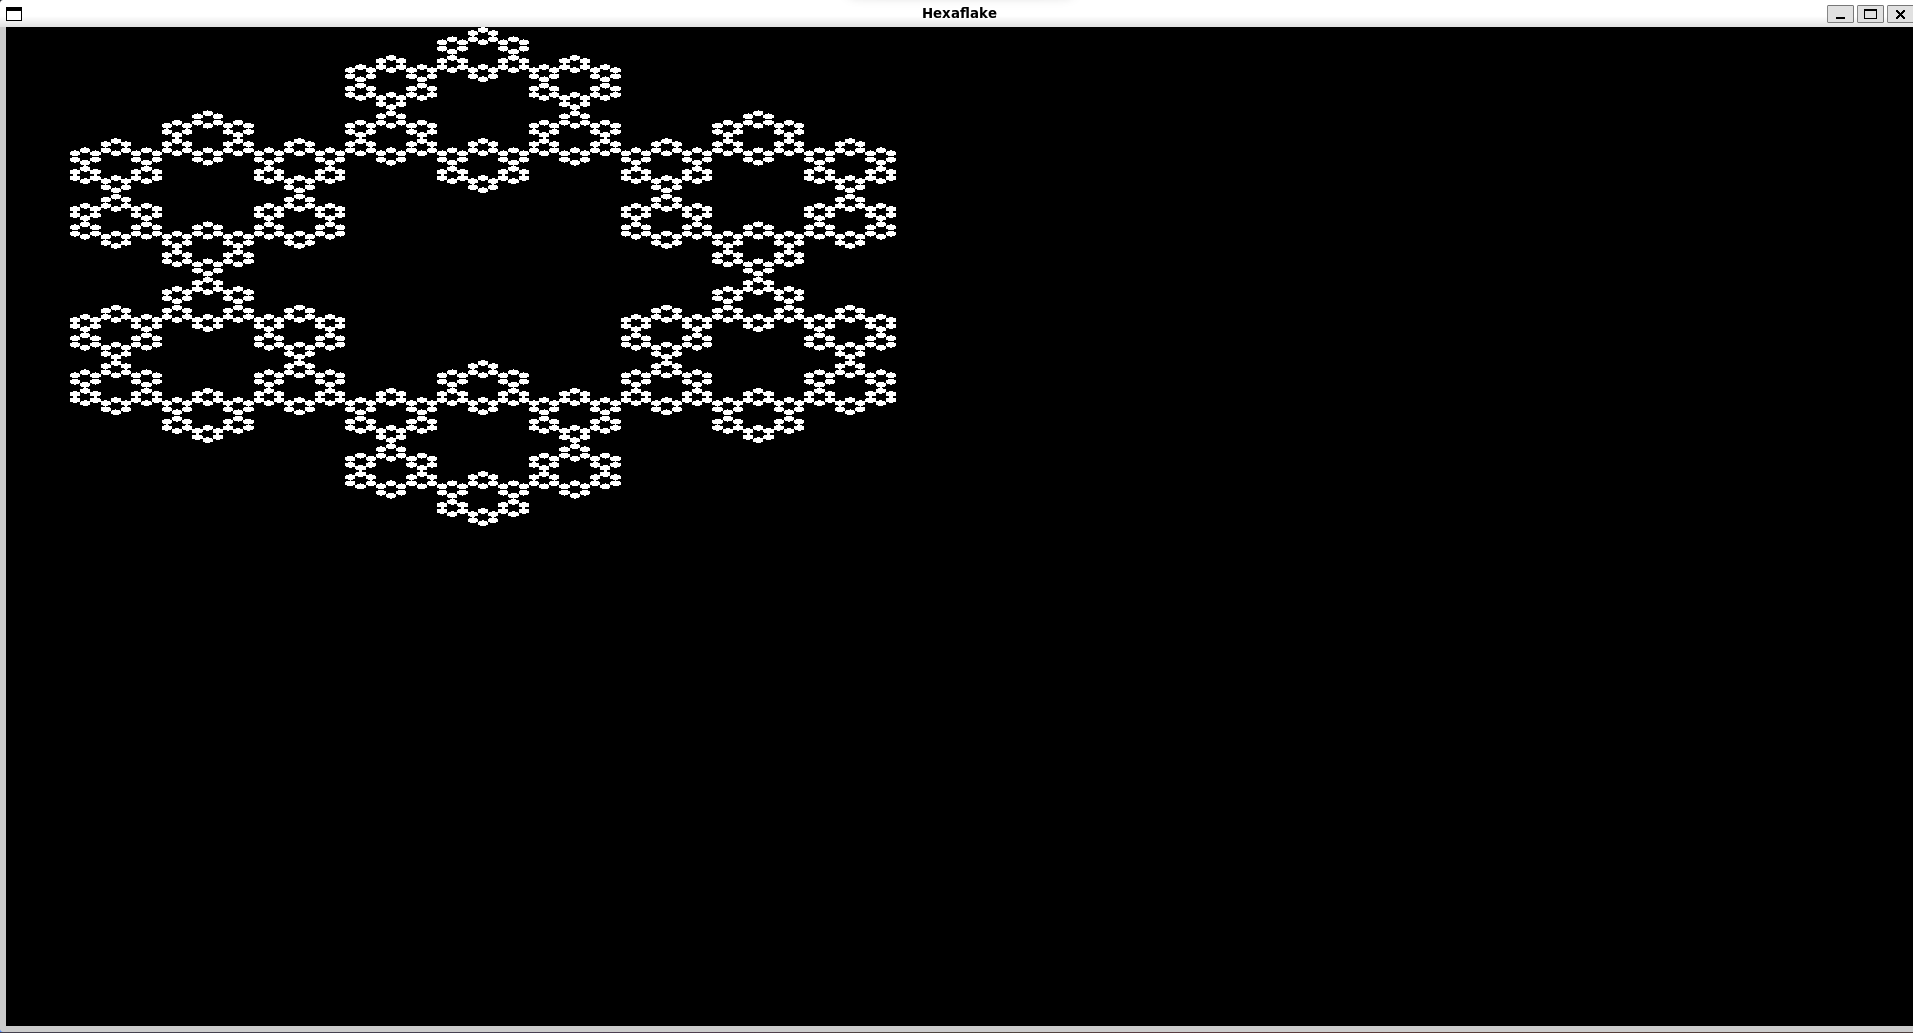
\includegraphics[width=6cm]{figures/screenshot.png}
	\caption{Window produced from running ps0}\label{fig:Hello}
\end{figure}


\subsection{What I accomplished}\label{sec:ps0:accomplish}

In this project, I was able to load a sprite with a .png file of Bijan Robinson, my top draft pick in fantasy football this season. Using the arrow keys, I was able to make this sprite move around the window, and with the space bar, the scale of the sprite would increase. The whole window could be reset using the 'R' key. I also added a text labeling Bijan Robinson.

\subsection{What I already knew}\label{sec:ps0:knew}

This being the first project of the semester, the only knowledge I had coming into this was the OOP paradigms we had learned in Computing 3, as well as my knowledge of various C++ libraries and practices.

\subsection{What I learned}\label{sec:ps0:learned}

This project introduced SFML library and I learned how to load textures to a sprite and interact with it based on keyboard strokes. Additionally, I implemented event-driven programming, where user inputs trigger specific actions. Moreover, it highlighted the significance of effective resource management, demonstrated by loading external assets like textures and fonts. 

\subsection{Challenges}\label{sec:ps0:challenges}

I didn't encounter any challenges, the goal of this program was relatively simple. However, one aspect of the program I didn't integrate that I probably should have, is adding boundaries on the window so the sprite isn't lost. But, the reset button prevents the program from having to be killed and restarted every time.

\subsection{Codebase}\label{sec:ps0:code}

\lstinputlisting[language=Make]{ps0/Makefile}
\lstinputlisting{ps0/main.cpp}

\newpage
